The SMs are the computational working blocks of the GPU.
It handles all tasks submitted to the GPU, which is executed in its sub components.
\Cref{fig:hw-sm} presents the hardware architecture of a basic SM, containing the key components which makes up the SM.
However keep in mind that this is not the complete content of all SMs, as the ones chosen presented here, is selected to provide an overview.

%TODO Update quality
\begin{figure}[H]
	\centering
	\fbox{
		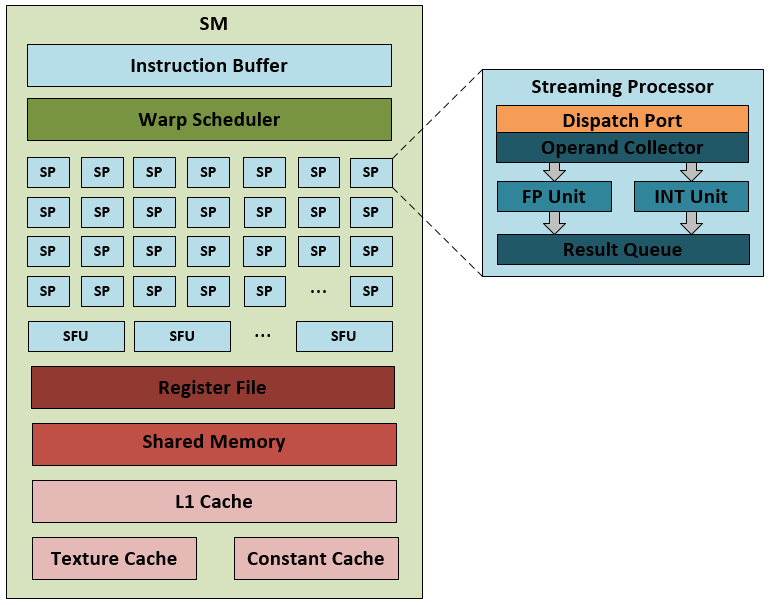
\includegraphics[width=0.8\textwidth]{figs/hw/hw-sm} }
	\caption{TBD}
	\label{fig:hw-sm}
\end{figure}

The key components and their functionality of SMs are:

\begin{itemize}
	\item \textbf{Streaming Processor (SM) -}  The most essential component of the SM is the SP, which is the basic computing element of the GPU.
	\Cref{sec-hw-streaming-processors} describes SP in detail, this section will cover its purpose within the SM.
	
	\item \textbf{Special Function Units (SFU) -} SFUs are a approximation units, which computes fast single-precision approximations of transcendental functions such as logarithm, exponential, sine and cosine \cite{Wilt2013}.
	Each of the SFUs also contains four floating-point multipliers that can offer extra throughput in addition to the SPs \cite{Li2016}.
	
	\item \textbf{Register File -} The Register File can be described as a chuck of memory used by the threads running on the SPs within a single SM. 
	The Register File runs at the same speed as the SP units, providing a minimum wait time on the register memory. 
	Instead of having a separate register dedicated to a single SP core, all SPs of a SM accesses the Register File, where registers are installed to be used by the threads of a SM.
	The data stored in the Register File is only visible to the thread which wrote it, and is deleted when the lifetime of the thread ends.
	Further information regarding the Register File can be found in \cref{sec-hw-memory-model}.
	
	\item \textbf{Shared Memory -} The Shared Memory is used to share data between threads running in the same block within the SM.
	Where the data stored in the Register File is only accessible by a single thread, the data stored in the Shared Memory can be accessed by multiple threads, which is further described in \cref{sec-hw-memory-model}.
		
	\item \textbf{Texture Cache -} The Texture Cache is a R/O used to access texture memory, allocated in the Global Memory.
	Texture memory is useful for data containing interpolation, which for example could be 2D or 3D lookup tables \cite{Cook2008}.
	
	\item \textbf{Constant Cache -} Just as the Texture Cache, the Constant Cache is R/O.
	Constant Cache is used for commonly used data, which is stored in the constant memory instead of global memory.
	This is done for the purpose of increasing performance in comparison to long latencies in conjunction with global memory accesses, which is further described in \cref{sec-hw-memory-model}.
	
	
	\item \textbf{L1 Cache -} 
	%First, let’s pick up on theintroduction of the L1 cache and what this means. An L1 (level one) cache is a cache present on a device and is the fastest cache type available.
	%The introduction of a cache makes it much easier for many programmers to write programs that work well on GPU hardware. It also allows for applications that do not follow a known memory pattern at compile time. However, to exploit the cache, the application either needs to have a sequential memory pattern or have at least some data reuse.
		
	\item  \textbf{Instruction Buffer \& Warp Scheduler -} The Instruction Buffer and Warp Scheduler are used to coordinate instructions and dispatch them to SPs.
	\Cref{sec-hw-warps} describes how these work in depth.
		
\end{itemize}

\Cref{fig:hw-sm-inside} presents an overview of how the different computational components of the SM is connected to the different memory components.
%TODO Tilføj mere generelt info om SM


%TODO Update quality
\begin{figure}[H]
	\centering
	\fbox{
		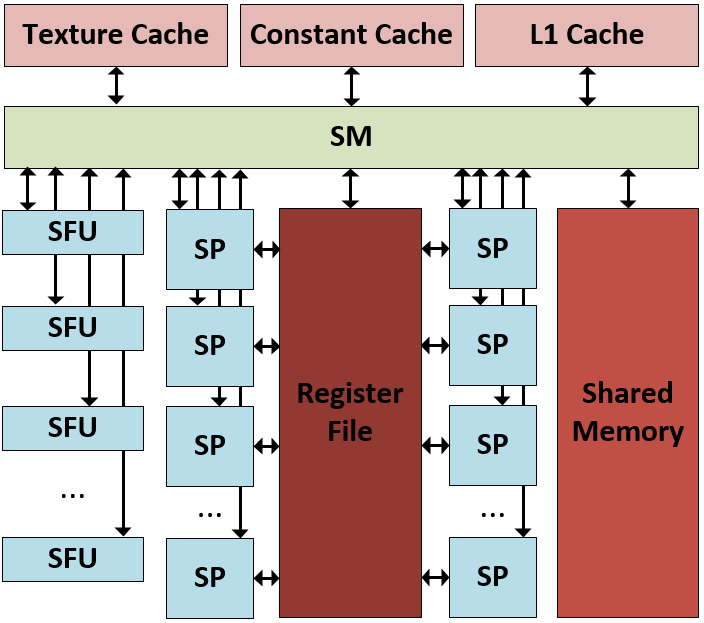
\includegraphics[width=0.6\textwidth]{figs/hw/hw-sm-inside} }
	\caption{TBD}
	\label{fig:hw-sm-inside}
\end{figure}







